\chapter{Contexte et objectifs du stage}

\section{Contexte du stage}

Le service reçoit chaque jour des appareils à contrôler, réparer ou remettre en état. Chaque appareil suit un parcours défini : retour et réception, désinfection, diagnostic, réparation, contrôle qualité, stock livrable puis livraison. L'enjeu est double : garantir la \textbf{sécurité} (un appareil ne doit pas repartir sans désinfection ni contrôle) et conserver l'\textbf{historique} de chaque appareil.

Les interventions portent sur des composants variés. Sur les concentrateurs d'oxygène, il s'agit notamment du compresseur, des électrovannes, des cartes électroniques et des colonnes à tamis moléculaire ; sur les appareils de ventilation, de l'écran tactile, des cartes électroniques, de la turbine et de la batterie. Ces composants alimentent le catalogue de pannes de l'application.

\begin{figure}[!htb]
\centering
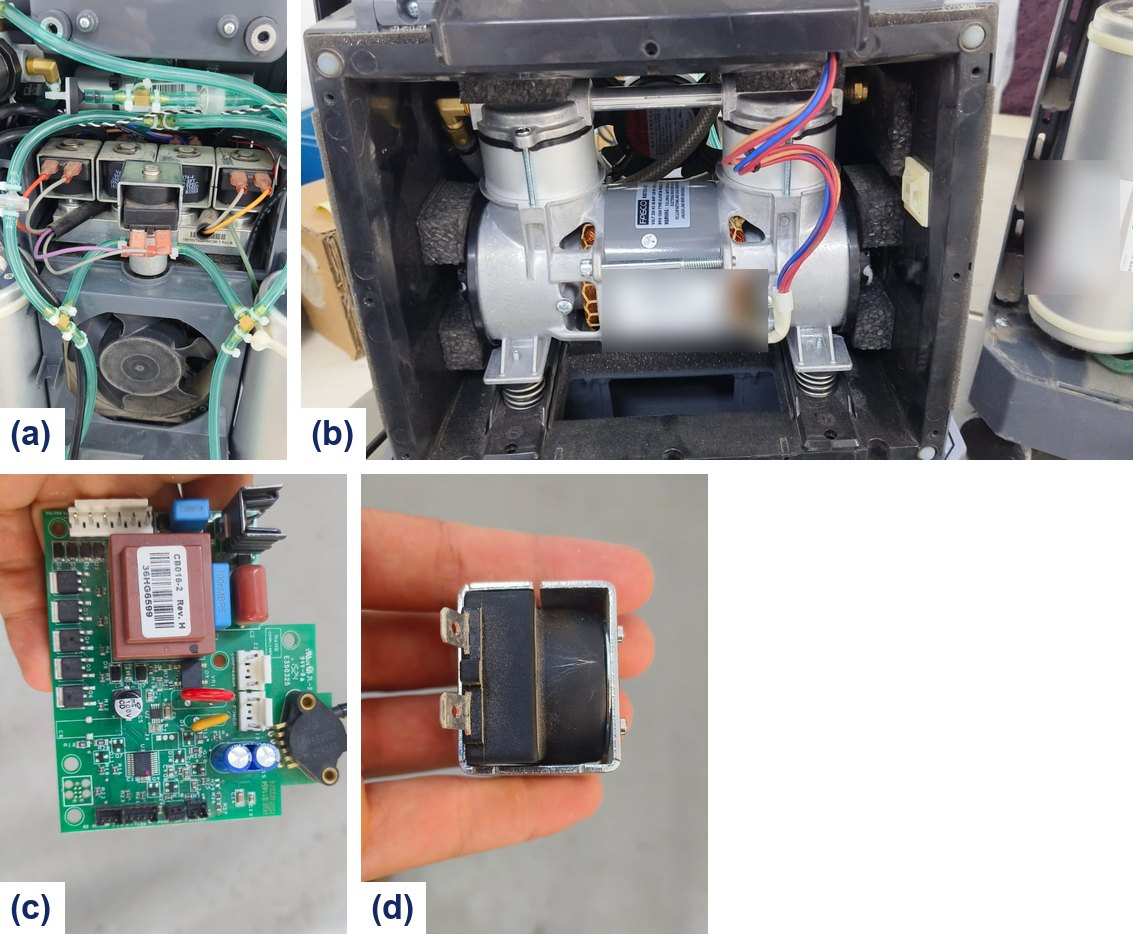
\includegraphics[width=14.0cm,height=12.0cm,keepaspectratio]{concentrateur_composants.jpg}
\caption{Composants d'un concentrateur d'oxygène : (a) vue interne, (b) compresseur, (c) carte électronique, (d) bobine d'électrovanne (étiquettes de série floutées)}
\end{figure}

\begin{figure}[!htb]
\centering
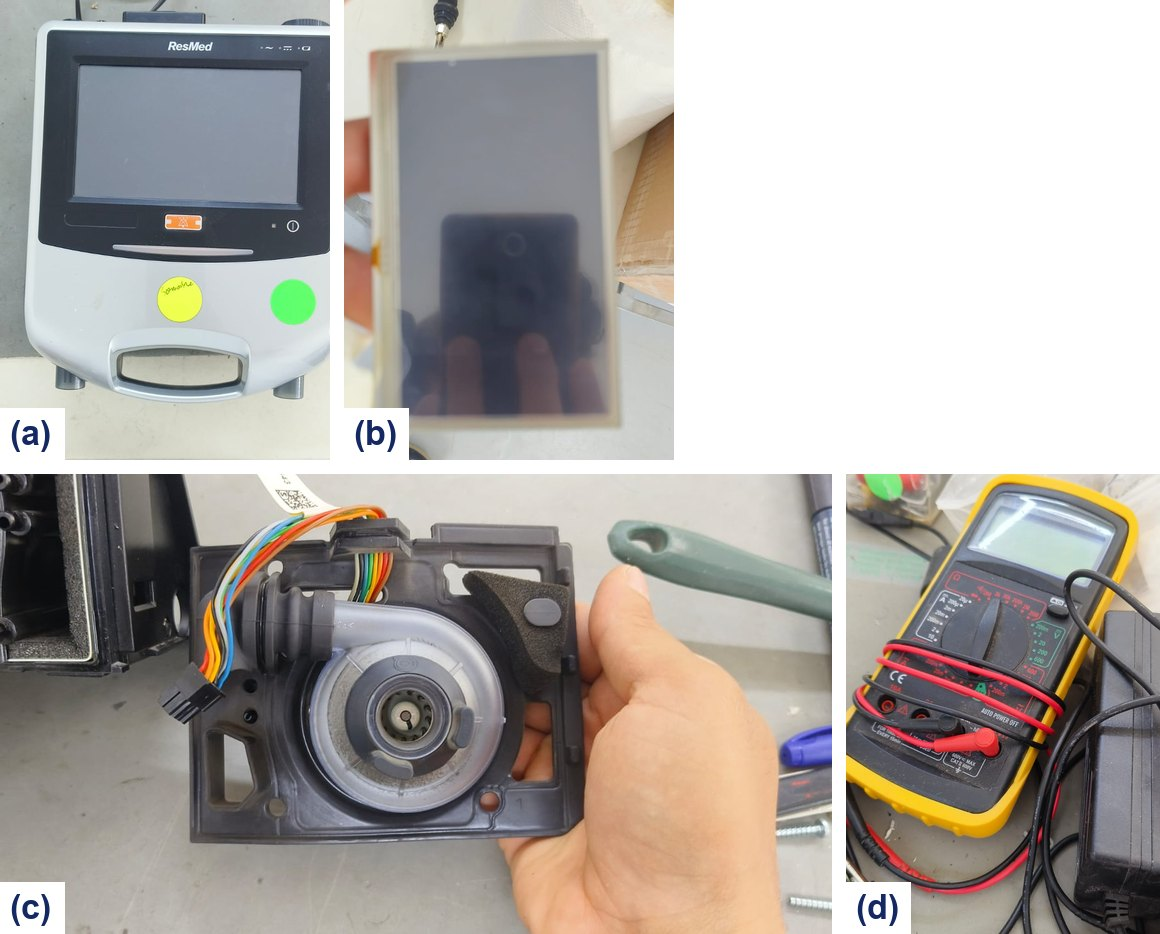
\includegraphics[width=14.0cm,height=12.0cm,keepaspectratio]{ventilation_composants.jpg}
\caption{Appareil de ventilation et composants : (a) appareil à écran tactile, (b) dalle tactile démontée, (c) turbine, (d) multimètre utilisé pour les contrôles}
\end{figure}

\section{Analyse de l'existant}

Trois supports étaient utilisés pour suivre l'activité. Par ailleurs, un progiciel de gestion (Microsoft Dynamics NAV) a été observé au poste de travail, utilisé pour les ordres de transfert ; le suivi technique des appareils restait en dehors de cet outil.

\subsection{Le journal de maintenance papier}

Un registre imprimé, intitulé \og{}Journal de maintenance des équipements O2, VNI, CPAP et respirateur\fg{} (référence 404, révision 1, propriétaire Air Liquide Tunisie), est rempli à la main pendant la journée sur un porte-bloc, une ligne par appareil. La figure suivante montre le registre le 14 juillet 2026.

\Needspace{22\baselineskip}
{\small\setstretch{1.05}\renewcommand{\arraystretch}{1.3}\arrayrulecolor{ALtexte}
\begin{longtable}{|>{\raggedright\arraybackslash}p{4.57cm}|>{\raggedright\arraybackslash}p{10.04cm}|}
\caption{Colonnes du journal de maintenance papier}\\
\hline
\rowcolor{ALbleu} \sffamily\bfseries\color{white} Colonne du registre & \sffamily\bfseries\color{white} Information notée \\ \hline
\endfirsthead
\caption[]{Colonnes du journal de maintenance papier (suite)}\\
\hline
\rowcolor{ALbleu} \sffamily\bfseries\color{white} Colonne du registre & \sffamily\bfseries\color{white} Information notée \\ \hline
\endhead
Année, Mois & Date de l'intervention \\ \hline
\rowcolor{ALgris} Équip. / type & Type d'équipement \\ \hline
N° série & Numéro de série de l'appareil \\ \hline
\rowcolor{ALgris} C.H & Compteur horaire de l'appareil \\ \hline
Pureté & Pureté de l'oxygène produit (concentrateurs) \\ \hline
\rowcolor{ALgris} Débit / pression & Mesures de débit ou de pression \\ \hline
Alarme sonore & Fonctionnement de l'alarme \\ \hline
\rowcolor{ALgris} Pannes & Pannes constatées \\ \hline
Doc de sortie PR & Document de sortie des pièces utilisées \\ \hline
\rowcolor{ALgris} Technicien & Technicien intervenant \\ \hline
Date sortie & Date de sortie de l'appareil \\ \hline
\end{longtable}
}

\begin{figure}[!htb]
\centering
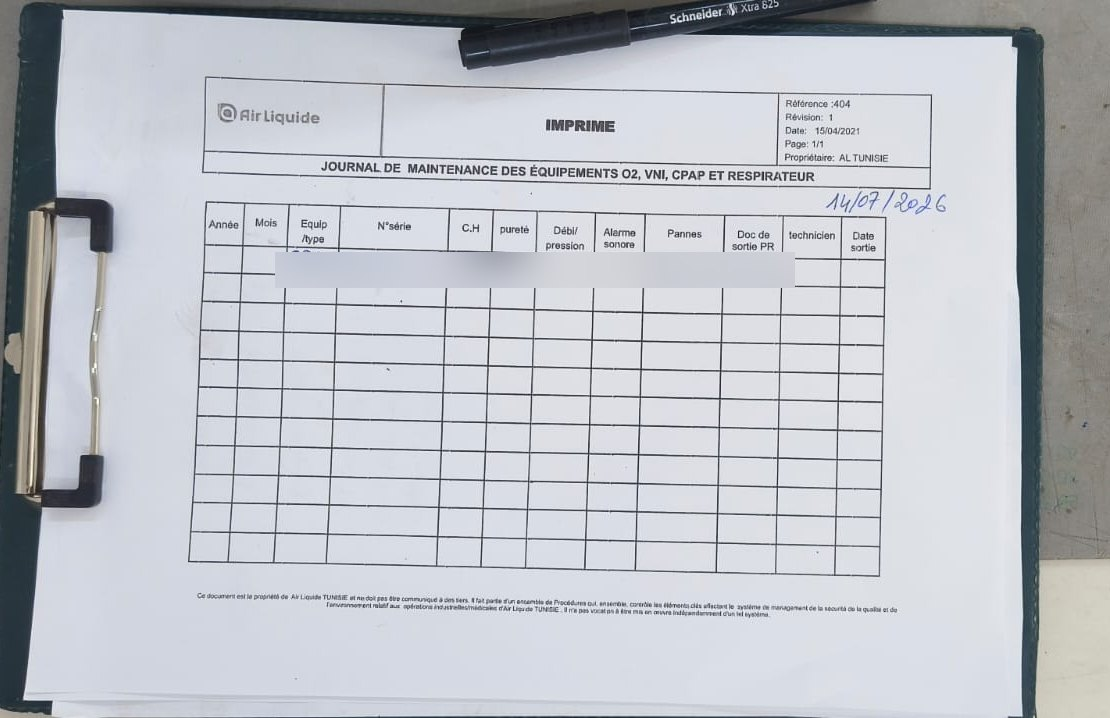
\includegraphics[width=13.5cm,height=10.0cm,keepaspectratio]{journal_papier.jpg}
\caption{Journal de maintenance papier du service (ligne manuscrite floutée)}
\end{figure}

\subsection{Le classeur Google Sheets \og{}GMAO v1\fg{}}

En fin de journée, les informations du papier étaient reportées dans un classeur Google Sheets. Il comporte plusieurs onglets, dont \textbf{RETURNS} (retours d'appareils), \textbf{DISINFECTION} (opérateur, statut, notes), \textbf{MAINTENANCE\_\allowbreak{}JOURNAL} (type de service, pièces, catégorie, propriété, heures de fonctionnement, pureté, dates de service), \textbf{LISTS}, \textbf{PM\_\allowbreak{}LOG} et \textbf{CM\_\allowbreak{}LOG}.

\begin{figure}[!htb]
\centering
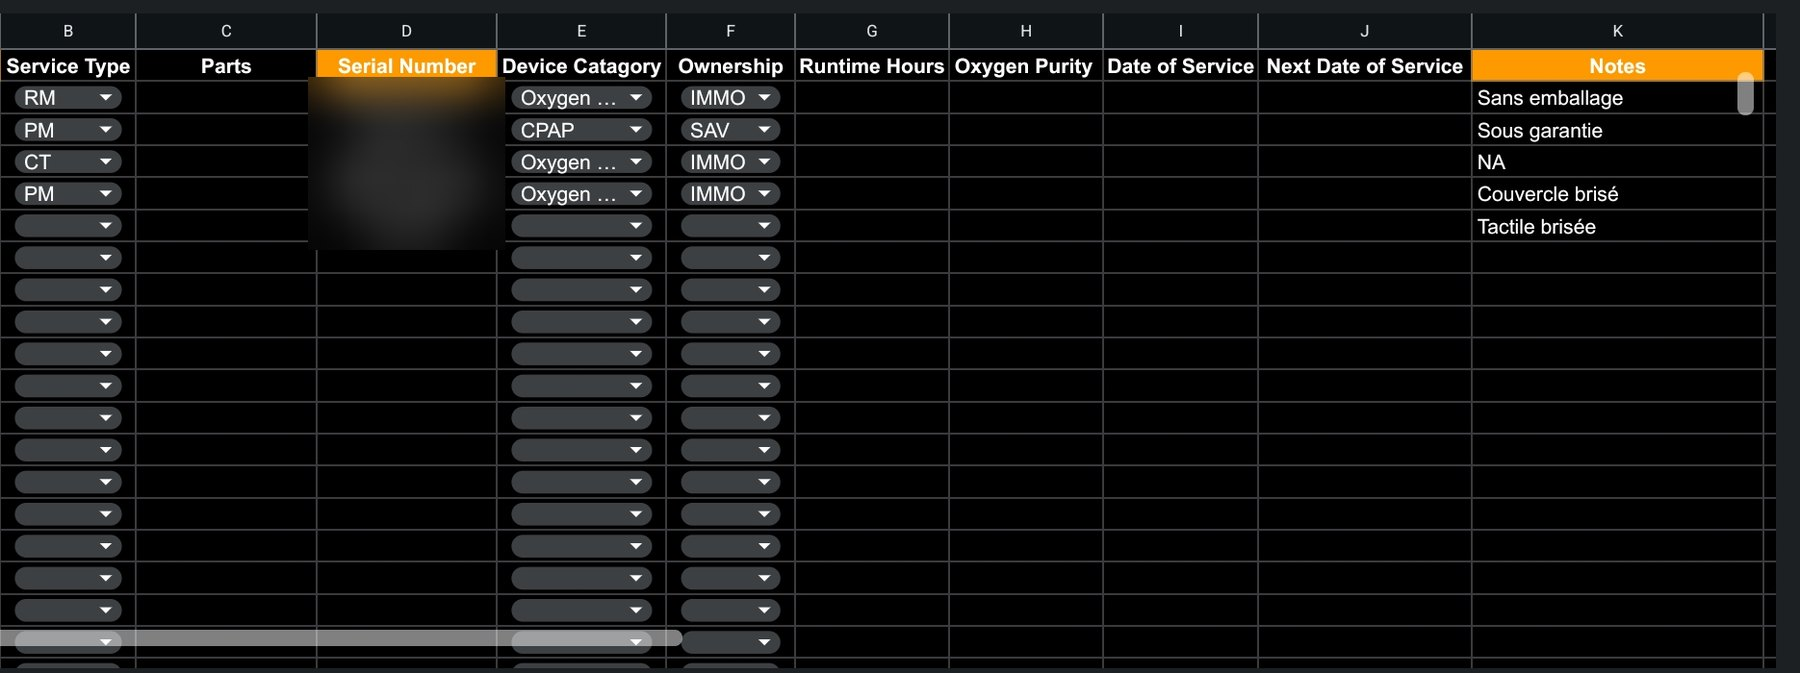
\includegraphics[width=15.5cm,height=7.0cm,keepaspectratio]{classeur_journal.jpg}
\caption{Onglet MAINTENANCE\_\allowbreak{}JOURNAL du classeur (numéros de série floutés)}
\end{figure}

\subsection{Le questionnaire de retour}

Avant l'arrivée d'un appareil, un questionnaire en ligne annonce le retour. Il recueille le numéro de série, l'état visuel (bon état, dégâts mineurs, réparation nécessaire, risque biologique), les accessoires manquants, des notes, un identifiant de retour et le statut biologique (normal, contamination importante, inconnu). Ses réponses alimentent l'onglet RETURNS du classeur.

\begin{figure}[!htb]
\centering
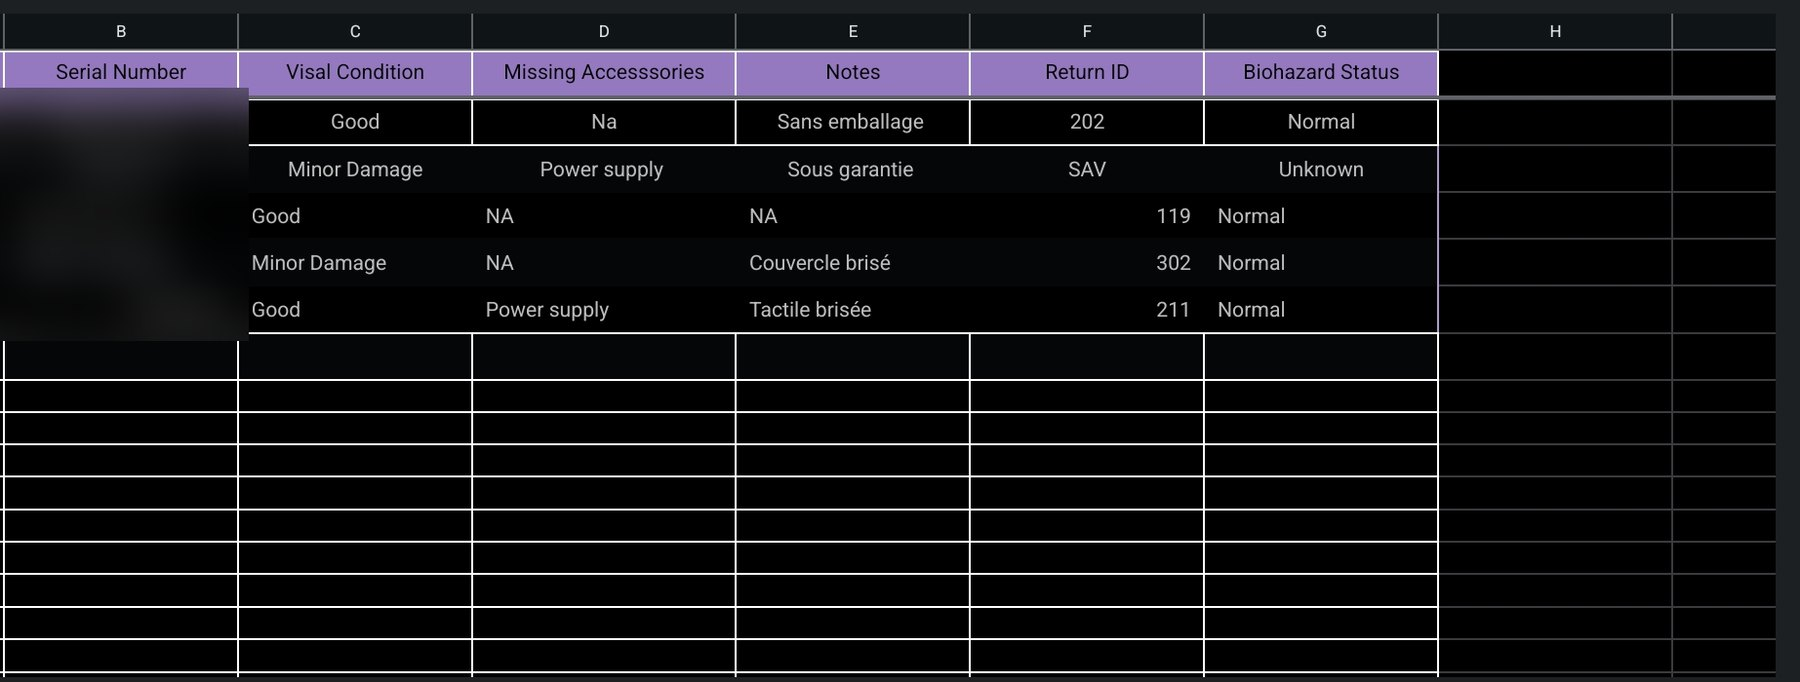
\includegraphics[width=15.5cm,height=6.5cm,keepaspectratio]{classeur_retours.jpg}
\caption{Onglet RETURNS : réponses au questionnaire de retour (numéros de série floutés)}
\end{figure}

\section{Problématique}

Ces supports présentent plusieurs limites, relevées dans le cahier des charges du projet : recherche lente des équipements, double saisie des informations, difficulté de suivre l'état des machines, absence de traçabilité complète et absence d'indicateurs de performance. La question centrale du stage est la suivante : \textbf{comment centraliser le suivi des appareils de leur retour à leur livraison, avec une traçabilité fiable et une saisie rapide pour les techniciens ?}

\section{Objectifs du stage}

\Needspace{22\baselineskip}
{\small\setstretch{1.05}\renewcommand{\arraystretch}{1.3}\arrayrulecolor{ALtexte}
\begin{longtable}{|>{\raggedright\arraybackslash}p{4.90cm}|>{\raggedright\arraybackslash}p{5.79cm}|>{\raggedright\arraybackslash}p{3.56cm}|}
\caption{Objectifs du stage et état de réalisation}\\
\hline
\rowcolor{ALbleu} \sffamily\bfseries\color{white} Objectif & \sffamily\bfseries\color{white} Critère de vérification & \sffamily\bfseries\color{white} Statut \\ \hline
\endfirsthead
\caption[]{Objectifs du stage et état de réalisation (suite)}\\
\hline
\rowcolor{ALbleu} \sffamily\bfseries\color{white} Objectif & \sffamily\bfseries\color{white} Critère de vérification & \sffamily\bfseries\color{white} Statut \\ \hline
\endhead
Enregistrer rapidement les retours & Formulaire de réception, reprise du questionnaire de retour & Réalisé \\ \hline
\rowcolor{ALgris} Une fiche de vie unique par appareil & Test : un appareil qui revient garde la même fiche & Réalisé, testé \\ \hline
Suivre chaque étape du cycle de maintenance & Workflow à 7 statuts, historique horodaté & Réalisé, testé \\ \hline
\rowcolor{ALgris} Empêcher les transitions incohérentes & Tests des règles de transition et des prérequis & Réalisé, testé \\ \hline
Enregistrer diagnostics, pannes, réparations, pièces & Catalogues et formulaires d'étape & Réalisé, testé \\ \hline
\rowcolor{ALgris} Contrôle qualité avec checklist & Checklist de 7 points, mesures & Réalisé, testé \\ \hline
Gérer le stock des appareils réparés & Mouvements d'entrée et de sortie & Réalisé, testé \\ \hline
\rowcolor{ALgris} Fournir tableau de bord et statistiques & Indicateurs et exports & Réalisé (tableau de bord, exports CSV) \\ \hline
Rapports PDF & Mentionnés au cahier des charges & Non réalisé (export CSV seulement) \\ \hline
\rowcolor{ALgris} Temps de saisie inférieur à une minute & Exigence du cahier des charges & Non mesuré \\ \hline
\end{longtable}
}

\section{Intérêt du stage dans ce contexte}

Le projet répond à un besoin réel du service. Il a permis de mettre en pratique la démarche complète d'un projet logiciel appliqué à la santé : recueil du besoin auprès des utilisateurs, conception, développement, tests et validation. Il se rattache directement à la formation TTIS, qui associe systèmes d'information et dispositifs médicaux.

